%!TEX root = ../dokumentation.tex

\chapter{Umsetzung}\label{cha:Umsetzung}
Nach Abschluss der Planung und der Durchführung des Setups, sowohl der \ac{VM} als auch der \ac{IDE}, kann die Entwicklung der Applikation beginnen. Im Folgenden werden die einzelnen Phasen der Entwicklung genauer dokumentiert.

Beginnend mit der Beschreibung der Infrastruktur sowie der Definition von Verarbeitungsprozessen. Anhand dieser orientiert sich die weitere Entwicklung der Anwendung. Abschließend wird ein Anwendungstest durchgeführt, bei welchem Logfiles unterschiedlicher Größe durch das Programm analysiert werden sollen. 

%<Allgemeine Beschreibung des Inhalts des Kapitels.>

\section{Infrastruktur \& Prozesse}
Vor Beginn der Entwicklung werden im Folgenden die Umgebung, in welcher die Applikation später ausgeführt werden soll, sowie der Anwendungsprozess, genauer definiert. 

Dies soll bei der Implementierung des Programms helfen, da durch die einzelnen Definitionen bereits eine grundlegende Idee geschaffen wird. Diese wird durch die eigentliche Implementierung komplettiert.

\subsection{Beschreibung der Infrastruktur}\label{subsec:Infrastruktur}
Obwohl Java als eine Plattform unabhängige Programmiersprache gesehen wird, spielt die Infrastruktur, in welcher die Anwendung ausgeführt werden soll, bei der Entwicklung eine entscheidende Rolle.

Durch die Infrastruktur wird indirekt die Art der Datenverarbeitung vorgegeben. Außerdem müssen potenzielle Einschränkungen, wie z.B. verfügbarer Speicherplatz oder maximale Übertragungsrate (falls Daten über ein Netzwerk ausgetauscht werden müssen), identifiziert werden.

Des Weiteren können, erst durch die Betrachtung der Umgebung, die Systeme ermittelt werden, welche für die Ausführung der Anwendung eventuell angepasst werden müssen (Installation zusätzlicher Software, Setzen von Berechtigungen, etc.).

Innerhalb der Infrastruktur werden drei verschiedene Serverarten unterschieden. Aktuell werden die Webseiten auf zwei physisch getrennten Webservern betrieben. Durch sie wird die Kommunikation zwischen den Clients und den \textit{Appservern} gesteuert (Annehmen von Requests und Senden des entsprechenden Response).

Die Inhalte für die einzelnen Seiten werden durch die \textit{Appserver} bereitgestellt. Die Anzahl dieser ist nicht festgelegt, um auf schwankende Anforderungen schneller regieren zu können. Steigt die Last auf das System, können weitere \textit{Appserver} der Infrastruktur hinzugefügt werden.

Der \textit{Infrastrukturserver} überwacht das gesamte System. Alle Informationen über den Zustand der Infrastruktur werden auf diesem Server konsolidiert. Dazu gehören ebenfalls die Logfiles. Diese werden, sowohl vom \textit{Web}- wie auch \textit{Appserver}, auf einem \ac{NFS} abgelegt. Die entsprechenden Verzeichnisse werden über einen mount dem \textit{Infrastrukturserver} zugänglich gemacht. 

Der \textit{Infrastrukturserver} muss über eine Hadoop Installation verfügen, auf welcher die Applikation ausgeführt werden muss. \autoref{fig:AufbauInfrastruktur} zeigt die beschriebene Infrastruktur. \\

\begin{figure}[h]
	\centering
	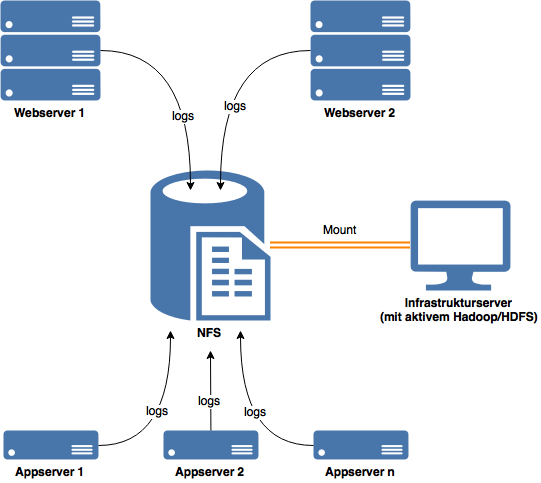
\includegraphics[width=.8\textwidth]{Infrastruktur.png}
	\caption{Aufbau der Infrastruktur}
	\label{fig:AufbauInfrastruktur}
\end{figure}

\subsection{Definition des Anwendungsprozesses}
Um die Entwicklung der Anwendung zu vereinfachen wird zunächst der vollständige Anwendungsprozess grob beschrieben. Die Beschreibung wird aus den in \autoref{sec:AnforderungenUndPLs} definierten Anforderungen und Produktleistungen abgeleitet.

%TODO: Einleitung schreiben/umschreiben
%<Einleitung noch nicht rund/komplett>

Nach dem Starten der Anwendung wird zunächst überprüft, ob beim Aufruf eine zusätzliche Konfiguration angegeben wurde. Ist dies der Fall, so wird die Konfiguration der Anwendung unter Verwendung dieser erzeugt. Anderenfalls wird die Standardkonfiguration verwendet.

Mit der erstellten Konfiguration wird mittels einer Initialisierungsfunktion ein \textit{Driver} für den Programmlauf erzeugt (\gls{Bootstrapping}). Der \textit{Driver} besitzt alle Informationen, welche für die Ausführung eines MapReduce Jobs benötigt werden.

Der \textit{Driver} wird anschließend durch den, vom Hadoop Framework bereitgestellten, \textit{ToolRunner} ausgeführt. Letztendlich wird die Anwendung mit dem vom \textit{ToolRunner} zurückgegebenen Statuscode beendet.

\autoref{fig:PAP_Main_main} zeigt den beschriebenen Prozess als \ac{PAP}. Die einzelnen Unterprozesse werden in den folgenden Kapiteln genauer betrachtet.\footnote{Die \acp{PAP} der Unterprozesse sind im Anhang (S. \pageref{subsec:PAPMainMain} bis \pageref{subsec:PAPDriverRun}) zu finden.}

\begin{figure}[h]
	\centering
	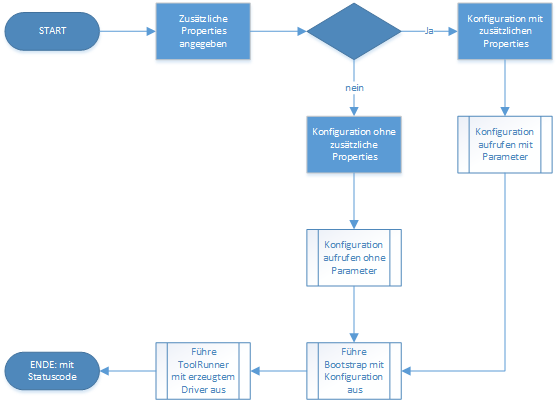
\includegraphics[scale=1]{PAP_Main_main.png}
	\caption{PAP für main Methode der Main Klasse}
	\label{fig:PAP_Main_main}
\end{figure}

%<Hier sollte der Prozess der Anwendung geplant werden. wo liegen die Daten? wie findet der zugriff statt? nach welchem schema sind sie abgelegt und benannt? Außerdem sollte klar werden wie die Informationen verarbeitet werden. ein großer map reduce oder eine Verkettung mehrerer mapper und reducer? Außerdem muss das Ausgabeformat festgelegt werden. Bzw. zwei alternativen. eine für wenn die Anwendung performant genug ist um als check skript zu laufen, und eine für den fall das nicht.>

\section{Die Konfigurationsschnittstelle}
Wie bereits bei der Beschreibung des Verarbeitungsprozesses gezeigt wurde, wird direkt nach dem Start der Anwendung eine Initialisierung vorgenommen. Hierbei soll die Umgebung so konfiguriert werden, dass die gewünschte Analyse durch die Anwendung ohne Probleme vorgenommen werden kann.

Die Konfiguration der Anwendung wird durch Dateien vom Typ \textit{.properties} vorgenommen. Diese werden von Java vollständig unterstützt. Für die Interpretation der Konfigurationsdateien wird auf die Klasse \textit{java.util.Properties} zurückgegriffen. Die Funktionsweise der Properties wird im Folgenden genauer betrachtet.

\subsection{Aufbau von Properties}
Die Konfigurationswerte werden in Properties Dateien als Schlüssel-Wert-Paare gespeichert. Die Trennung kann hierbei durch einen Doppelpunkt oder Gleichheitszeichen erfolgen. Des weiteren ist es möglich, Platzhalter bei den Werten zu definieren, welche später durch Variablen ersetzt werden können. Außerdem ist es möglich, zum besseren Verständnis, die Datei um Kommentare zu erweitern. Jede Zeile, welche mit einem Hash oder Ausrufezeichen beginnt, wird als Kommentar gesehen, und von der Anwendung nicht interpretiert. \autoref{lis:AuszugDefaultProperties} zeigt einen Auszug aus der \textit{default.properties} Datei. \\

\begin{lstlisting}[language=Bash,caption=Auszug aus default.properties,label=lis:AuszugDefaultProperties]
###
# Default properties for Logfileanalyzer.
# Properties can be extended by user defined properties.
# Never change this file to fit one case.
#

# Set mode for execution (DEBUG, TEST, LIVE)
lfa.runmode         : DEBUG

# Runtime properties
lfa.logger.handlers : {0}

[...]
\end{lstlisting}

Grundsätzlich sind alle Konfigurationen vom Typ \textit{String}. Es ist, nativ, nicht möglich, direkt einen Wert in einem anderen Datentyp zu definieren. Falls eine Typenkonvertierung notwendig ist, muss diese manuell durchgeführt werden.

In Java stellt die Klasse \textit{Properties}, welche Teil des \textit{java.util} Paketes ist, alle benötigten Methoden bereit. Um die Konfiguration der Anwendung zu vereinfachen, wurde die Klasse \textit{LFAConfiguration}\footnote{Der Name \textit{LFAConfiguration} wurde bewusst gewählt, da der Name \textit{Configuration} bereits von einer Klasse des Hadoop Frameworks verwendet wird.} im Paket \textit{com.hszuesz.logfileanalyzer} erzeugt. Diese leitet sich aus der Klasse \textit{Properties} ab, und stellt Erweiterungen zum Einlesen mehrerer Konfigurationsdateien bereit. Dies ist notwendig, um eine stufenweise Konfiguration der Anwendung zu realisieren.

Da die Anwendung später innerhalb des Hadoop Frameworks ausgeführt wird, müssen die Konfigurationsdateien ein Teil der, durch Maven erzeugten, JAR-Datei sein. Dies wird durch eine Ergänzung in der \textit{pom.xml} innerhalb des \textit{build} Knotens sichergestellt (siehe \autoref{lis:POMErgänzung}). \\

\begin{lstlisting}[language=XML,caption=pom.xml Ergänzung für Konfigurationsdateien,label=lis:POMErgänzung]
[...]
<resources>
	<resource>
		<directory>conf</directory>
		<includes>
			<include>*.properties</include>
		</includes>
	</resource>
</resources>
[...]
\end{lstlisting}

\subsection{Beschreibung der Konfigurationsstufen}
Die Konfiguration der Anwendung wird in drei Stufen durchgeführt. Dies soll die Komplexität der Konfigurationsdateien reduzieren, indem die individuellen Anpassungen für jede Ausführung des Programms gekapselt und immer gleiche Einstellungen ausgelagert sind.

Die erste Stufe bilden die sog. Core-Properties, welche in der Datei \textit{core.properties} hinterlegt sind. Wie der Name bereits erkennen lässt, handelt es sich hierbei um grundlegende Einstellungen, welche den Kern der Anwendung beeinflussen. Dazu gehört z.B. die Konfiguration der verschiedenen \textit{RUNMODES} oder Pfade zu weiteren wichtigen Dateien, wie den Default- oder Logger-Properties. Ein Überschreiben dieser Einstellungen ist nicht möglich.

Die zweite Stufe bildet die Defaults. Hier werden alle Konfigurationen vorgenommen, welche für eine Standardausführung der Anwendung benötigt werden. Alle Einstellungen, welche in der \textit{defaults.properties} Datei hinterlegt sind, können durch den Anwender verändert werden.

Die dritte und letzte Stufe bilden die User-Properties. Beim Start der Anwendung kann der Pfad zu einer individuellen Properties-Datei übergeben werden. In dieser können die Einstellungen, welche durch die Defaults vorgenommen wurden, ergänzt und  überschreiben werden.

Der Prozess für die Verarbeitung der einzelnen Stufen wird im \ac{PAP} der \textit{LFAConfiguration} verdeutlicht, welcher im Anhang zu finden ist.\footnote{\ac{PAP} für \textit{LFAConfiguration} im Anhang, S. \pageref{subsec:PAPLFAConfiguration}}

%<Beschreibung wie Properties programmiert werden. Wie werden diese in der Anwendung umgesetzt? Welche Rolle spielen Properties für den generischen Teil der Anwendung?>

\subsection{Logger Konfiguration}
Ein weiteres Modul, welches durch die Konfigurationsschnittstelle beeinflusst wird, ist der Logger. Die Anwendung verwendet den Standard Logger von Java, welcher sich über eine externe Properties Datei beliebig einstellen lässt.

Es gibt zwei Möglichkeiten die Arbeitsweise des Loggers zu beeinflussen. Die erste bildet der sog. \textit{Rumode}, welcher sich über die Property \textit{lfa.runmode} setzen lässt. Es wird unterschieden zwischen \textit{DEBUG}, \textit{TEST} und \textit{LIVE}. \autoref{tbl:LoggerSettingsRunmode} zeigt die Voreinstellungen des Loggers, für die unterschiedlichen Runmodes. Diese Einstellungen können durch eine zusätzliche Konfigurationsdatei individuell angepasst werden. 

\begin{table}[h]
	\centering
	\begin{tabular}{| l | l | l | l |}
		\hline
		\rowcolor[HTML]{3531FF} 
		\multicolumn{1}{|l|}{\cellcolor[HTML]{4F88BB}{\color[HTML]{FFFFFF} {\bf Runmode}}} & \multicolumn{1}{l|}{\cellcolor[HTML]{4F88BB}{\color[HTML]{FFFFFF} {\bf Handlers}}} & \multicolumn{1}{l|}{\cellcolor[HTML]{4F88BB}{\color[HTML]{FFFFFF} {\bf Loglevel}}} & \multicolumn{1}{l|}{\cellcolor[HTML]{4F88BB}{\color[HTML]{FFFFFF} {\bf Formatter}}} \\ \hline
		\textbf{DEBUG} & ConsoleHandler & ALL & SimpleFormatter \\  \hline
		\textbf{TEST} & FileHandler & WARNING & SimpleFormatter \\ \hline
		\textbf{LIVE} & FileHandler & SEVERE & SimpleFormatter \\  \hline
	\end{tabular}
	\caption{Logger Einstellungen für die einzelnen Runmodes\footnotemark}
	\label{tbl:LoggerSettingsRunmode}
\end{table}
\footnotetext{Die Angaben in den Spalten \textit{Handlers} und \textit{Formatter} haben noch den zusätzlichen Prefix \\ \textit{java.util.logging.}, um die expliziten Klassen zu definieren.}

Aus den einzelnen Konfigurationsdateien werden die endgültigen Einstellungen zusammengestellt und über den \textit{LogManager} gesetzt. Für den \textit{FileHandler} wird zusätzlich ein Pattern definiert, welches den Speicherort und Dateinamen des Logfiles angibt. \autoref{lst:BeispielConfLogger} zeigt ein Beispiel für eine Logger Konfiguration. Im angegebenen Pattern sind zwei Platzhalter definiert. Die Variable \textit{\%h} wird mit dem Home-Verzeichnis des aktiven Users ersetzt, \textit{\%u} mit einer Identifikationsnummer. \\

\begin{lstlisting}[language=Java,caption=Beispiel Konfiguration für den Logger,label=lst:BeispielConfLogger]
handlers=java.util.logging.FileHandler
java.util.logging.FileHandler.level=ALL
java.util.logging.FileHandler.formatter=java.util.logging.SimpleFormatter
java.util.logging.FileHandler.pattern=%h/scripts/default_%u.log
\end{lstlisting}

%<Beschreibung wie der Logger in Java funktioniert und wie dieser hier eingesetzt wird. Speziell die Konfiguration über die logger.properties datei hervorheben.>

\subsection{Konfiguration der Anwendung}
Um eine Vielzahl an unterschiedlichen Analysen durchführen zu können, sind die einzelnen, in \autoref{subsec:DatenflussMapReduce} beschriebenen Komponenten über Properties konfigurierbar. Gemäß der Architektur der Anwendung, sind auch die Einstellungen in unterschiedlichen Gruppen gekapselt.

\begin{table}[h]
	\centering
	\begin{tabularx}{\textwidth}{| l | l | l | X |}
		\hline
		\rowcolor[HTML]{3531FF} 
		\multicolumn{1}{l|}{\cellcolor[HTML]{4F88BB}{\color[HTML]{FFFFFF} {\bf Gruppe}}} &
		\multicolumn{1}{l|}{\cellcolor[HTML]{4F88BB}{\color[HTML]{FFFFFF} {\bf Property}}} &
		\multicolumn{1}{l|}{\cellcolor[HTML]{4F88BB}{\color[HTML]{FFFFFF} {\bf Standardwert}}} & \multicolumn{1}{l|}{\cellcolor[HTML]{4F88BB}{\color[HTML]{FFFFFF} {\bf Beschreibung}}} \\ \hline
		lfa.driver & .mapper & \footnotemark[1].mapper.PatternMapper & Klasse für den Mappingvorgang \\ \cline{2-4}
		 & .reducer & \footnotemark[1].reducer.SumReducer & Klasse für den Reducevorgang \\ \hline
		*.input & .format & \footnotemark[2].input.TextInputFormat & Klasse für die Interpretation des Inputs \\ \hline
		*.output & .key & \footnotemark[3].Text & Klasse für den Datentyp des Schlüssels \\ \cline{2-4}
		 & .value & \footnotemark[3].IntWritable & Klasse für den Datentyp des Wertes \\ \cline{2-4}
		 & .format & \footnotemark[2].output.TextOutputFormat & Klasse für die Formatierung des Outputs \\ \hline
		*.job & .name & Logfileanalyzer & Name für den MapReduce Job \\ \hline
		lfa.mapper & .* &  & Zusätzliche Properties für den Mapper \\ \hline
		lfa.reducer & .* &  & Zusätzliche Porperties für den Reducer \\ \hline
	\end{tabularx}
	\caption{Properties zur Steuerung der Analyse}
	\label{tbl:AppProperties}
\end{table}
\footnotetext[1]{com.hszuesz.logfileanalyzer}
\footnotetext[2]{org.apache.hadoop.mapreduce.lib}
\footnotetext[3]{org.apache.hadoop.io}

\autoref{tbl:AppProperties} zeigt die wichtigsten Properties zur Steuerung der Anwendung mit ihren jeweiligen Standardwerten. Die Werte können durch Setzen der Einstellungen in den User Properties verändert werden. Soll z.B. statt einer Summe der Durchschnitt der Werte für einen Schlüssel ermittelt werden, so ist die Property \textit{lfa.driver.reducer} auf den Wert \textit{com.hszuesz.logfileanalyzer.reducer.AverageReducer} zu setzen. Es findet keine Überprüfung der Werte Statt. Die Angabe von ungültigen Konfigurationseinstellungen (z.B. einer nicht bekannten Klasse) führt zum Programmabsturz.

Die Einstellungen \textit{lfa.mapper} sowie \textit{lfa.reducer}, dienen der weiteren Konfiguration der jeweiligen Klassen. So wird beispielsweise über \textit{lfa.mapper.pattern.key} der reguläre Ausdruck für den Pattern Mapper festgelegt.

%\section{Grundlagen für Datenverarbeitung}
%<Beschreibung der Entwicklung für die Grundlagen zur Datenverarbeitung. Welche Klassen werden dabei verwendet? Welches System liegt dahinter? Warum dieses System? Dabei nicht nur auf die Speicherung von Daten eingehen sondern auch auf das Lesen von Dateien.>

%\section{Bestimmung des Aufbaus der Logfiles}
%<Wie sehen die Logfiles aus? Welche Formate haben sie? Welche rolle spielen diese bei der Datenverarbeitung? Welche Informationen sind die richtigen Informationen?>

\section{Implementierung von MapReduce}
Nachdem alle Grundlagen der Anwendung fertiggestellt wurden kann mit der Entwicklung des Kernstückes begonnen werden, der Implementierung von MapReduce. Der Verarbeitungsprozess innerhalb des MapReduce Modells wurde bereits in \autoref{subsec:DatenflussMapReduce} beschrieben. Nachfolgend wird sowohl die Funktionsweise als auch die Entwicklung der einzelnen Module der Anwendung beschrieben.

\subsection{Funktion von Bootstrap \& Driver}
Durch den generischen Ansatz der Anwendung muss jeder Programmlauf initialisiert werden (auch als \gls{Bootstrapping} bezeichnet). Dies wird durch die Methode \textit{init} der Klasse \textit{Bootstrap} durchgeführt. Die zuvor erstellte Instanz der Klasse \textit{LFAConfiguration} wird hierfür an die Methode übergeben. Basierend auf den gesetzten Properties wird eine Instanz der Klasse \textit{Driver} erzeugt (siehe \autoref{lst:BootstrapInit} oder \ac{PAP}\footnote{\ac{PAP} für \textit{Bootstrap:init() im Anhang, S. \pageref{subsec:PAPBootstrapInit}}}).

Dem \textit{Driver} werden zunächst alle Klassen mitgeteilt, welche zur Ausführung eines Jobs essentiell notwendig sind. Hierzu gehören die Klassen für \textit{InputFormat}, \textit{OutputFormat}, \textit{OutputKey}, \textit{OutputValue}, \textit{Mapper} und \textit{Reducer}. Die gesetzten Werte sind vom Typ \textit{Class<?>}. Es werden keine Instanzen der Klassen erzeugt. Ebenfalls notwendig für die Ausführung eines Jobs ist das Setzen eines Namens.

\newpage
Zuletzt wird eine Iteration über alle Schlüssel der Konfiguration durchgeführt, um zusätzliche Properties an den \textit{Driver} zu übergeben. Diese erweiterten Einstellungen werden vor Ausführung des Jobs in eine Instanz der Klasse \textit{org.apache.hadoop.conf.Configuration} geschrieben. Bei diesen Properties handelt es sich um Einstellungen, welche von den einzelnen Modulen des MapReduce Modells verwendet werden (z.B. ein regulärer Ausdruck für die \textit{Mapper} Klasse).\\

\begin{lstlisting}[language=Java,caption=Auszug der Methode \textit{Bootstrap:init()},label=lst:BootstrapInit]
public static Driver init(LFAConfiguration objConfiguration) {
	[...]
	
	// Set class to use for InputFormat
	objDriver.setClsInputFormatClass(Class.forName(objConfiguration.getProperty("lfa.driver.input.format")));
	
	[...]
	
	// Set classes for mapper and reducer
	objDriver.setClsMapperClass(Class.forName(objConfiguration.getProperty("lfa.driver.mapper")));
	
	[...]
	
	Set<String> setKeys = objConfiguration.stringPropertyNames();
	
	// Extract additional properties for the MapReduce job
	for (String strKey : setKeys) {
		if (strKey.contains("lfa.mapper.") || strKey.contains("lfa.reducer.") || strKey.contains("lfa.driver.add.")) {
			objDriver.setAdditionalConfiguration(strKey, objConfiguration.getProperty(strKey));
		}
	}
	
	[...]
}
\end{lstlisting}

Die Klasse \textit{Driver} leitet sich von \textit{org.apache.hadoop.conf.Configured} ab und implementiert das Interface \textit{org.apache.hadoop.util.Tool}. Von der Klasse \textit{Configured} werden alle notwendigen Methoden und Attribute geerbt, welche für die Verwendung der, durch das Hadoop Framework gestellte und interpretierte, Konfiguration notwendig sind. Durch das Interface wird wiederum die Implementierung der Methode \textit{run()} vorgegeben.

Diese Methode, welche später durch den \textit{ToolRunner} aufgerufen wird, erstellt und konfiguriert einen neuen Job, um diesen auszuführen und seinen Statuscode zurück zu geben. Hier werden alle, durch die \textit{Bootstrap:init()} Methode gesetzten Einstellungen, an den Job übergeben. Dieser Umweg ist notwendig, da ein Job mit einer Instanz von \textit{import org.apache.hadoop.conf.Configuration} erzeugt werden muss. Diese steht erst nach Ausführung durch den \textit{ToolRunner} zu Verfügung.

Dieser Konfigurationsklasse werden ebenfalls die zusätzlichen Einstellungen übergeben, sofern diese vorhanden sind. Das übergebene Array enthält die Pfade für den Input und Output des Jobs, welche der Klasse \textit{FileInputFormat} und \textit{FileOutputFormat} hinzugefügt werden. \autoref{lst:AuszugRunMethode} zeigt einen Auszug der \textit{run} Methode (siehe auch \ac{PAP}\footnote{\ac{PAP} für \textit{Driver.run()} im Anhang, S. \pageref{subsec:PAPDriverRun}}) \\

\begin{lstlisting}[language=Java,caption=Auszug der \textit{run()} Methode,label=lst:AuszugRunMethode]
public int run(String[] arrArguments) throws Exception {
	Configuration objConf = this.getConf();
	
	if (this.mapAdditionalConfigurations.size() > 0) {
		for (String strKey : this.mapAdditionalConfigurations.keySet()) {
			objConf.set(strKey, this.mapAdditionalConfigurations.get(strKey));
		}
	}
	
	Job objJob = new Job(objConf, this.strJobName);
	
	[...]
	
	FileInputFormat.addInputPath(objJob, new Path(arrArguments[0]));
	objJob.setInputFormatClass(this.clsInputFormatClass);
	
	FileOutputFormat.setOutputPath(objJob, new Path(arrArguments[1]));
	objJob.setOutputFormatClass(this.clsOutputFormatClass);
	
	return objJob.waitForCompletion(true) ? 0 : 1;
}
\end{lstlisting}

\newpage
\subsection{Einblick in die Funktion von Input-/OutputFormat}
Klassen, welche das Interface \textit{InputFormat} implementieren (oder sich von Klassen, welche das Interface implementieren, ableiten), geben vor, wie die Eingabedaten gelesen werden müssen. \autoref{tbl:InputFormatKlasses} zeigt die bestehenden \textit{InputFormat} Klassen sowie deren Arbeitsweise.

\begin{table}[h]
	\centering
	\begin{tabularx}{\textwidth}{| l | X | X | X |}
		\hline
		\rowcolor[HTML]{3531FF} 
		\multicolumn{1}{|l|}{\cellcolor[HTML]{4F88BB}{\color[HTML]{FFFFFF} {\bf Klasse}}} & \multicolumn{1}{l|}{\cellcolor[HTML]{4F88BB}{\color[HTML]{FFFFFF} {\bf Beschreibung}}} & \multicolumn{1}{l|}{\cellcolor[HTML]{4F88BB}{\color[HTML]{FFFFFF} {\bf Key}}} & \multicolumn{1}{l|}{\cellcolor[HTML]{4F88BB}{\color[HTML]{FFFFFF} {\bf Value}}} \\ \hline
		\textit{TextInputFormat} & Liest Zeile für Zeile einer Textdatei & Byte-Offset der Zeile & Inhalt der Zeile \\  \hline
		\textit{KeyValueInputFormat} & Parst Schlüssel und Wert aus einer Zeile & Text bis zum ersten Tab & Rest der Zeile \\ \hline
		\textit{SequenceFileInputFormat} & Hadoop-spezifisches Binärformat & Benutzerdefiniert & Benutzerdefiniert \\  \hline
	\end{tabularx}
	\caption{Bestehende InputFormat-Klassen für Map-Reduce\footnotemark}
	\label{tbl:InputFormatKlasses}
\end{table}
\footnotetext{\cite[S. 61.]{Freiknecht.2014}}

Generell ist es möglich, jegliche Form von Daten, mit MapReduce zu analysieren. Handelt es sich jedoch nicht um textbasierte Dateiformate (wie z.B. Bilder oder Dateien im \ac{PDF}), ist die Entwicklung individueller Klassen notwendig.

Zudem teilt Hadoop besonders große Dateien (mehrere \ac{GB}). in sog. \textit{Splits}, um die Verarbeitung, wenn dies für ein gegebenes Dateiformat möglich ist, in kleineren Einheiten auf verschiedene Knoten im Cluster zu verteilen. \flqq Gerade wenn Dateien Metadaten enthalten (z.B. Farbpaletten in Bildern oder Informationen über Künstler in MP3s), dann ist die Datei sicherlich nicht in einem sequenziell lesbaren Format geschrieben.\frqq\footcite[S. 110]{Freiknecht.2014}

Daher muss bei der Verarbeitung einer Datei immer bedacht werden, ob es möglich ist, diese sequenziell zu verarbeiten. Wenn dies nicht der Fall ist, muss eine entsprechende Klasse implementiert werden, um Fehler bei der Analyse zu vermeiden.

In einem Beispiel verwendet Jonas Freiknecht \acp{PDF} als Eingabedaten. Da es sich bei \acp{PDF} um Dateien in einem Binärformat handelt, muss eine entsprechende Klasse implementiert werden. \autoref{lst:PDFInputFormat} zeigt die von Freiknecht entwickelte Klasse \textit{PDFInputFormat}. Die in Zeile 15 definierte Methode \textit{isSplittable()}, welche den boolean Wert \textit{false} zurückgibt, verhindert, dass die Datei in kleinere Einheiten unterteilt wird. \\

\begin{lstlisting}[language=Java,caption=Die Klasse PDFInputFormat, title=\autoref*{lst:PDFInputFormat}: Die Klasse PDFInputFormat\protect\footnotemark,label=lst:PDFInputFormat]
public class PDFInputFormat extends FileInputFormat<Text, Text> {
	
	// Eingabe Key und Value müssen den Datentypen des Mappers
	// entsprechen
	@Override
	public RecordReader<Text, Text> createRecordReader(InputSplit split, TaskAttemptContext context) throws IOException, InterruptedException {
	
		// Der Record-Reader muss [...] Datentypen des Mappers entsprechen,
		// andernfalls wird [...] auf einen Typ-Missmatch hingewiesen.
		return new PDFLineRecordReader();
	}
	
	// Verbiete es, PDF-Dateien zu splitten
	@Override
	protected boolean isSplittable(JobContext context, Path filename) {
		return false;
	}
	
}
\end{lstlisting}
\footnotetext{\cite[S. 115.]{Freiknecht.2014}}

Ähnlich zu den Klassen, welche das \textit{InputFormat} Interface implementieren, gibt es das Interface \textit{OutputFormat}, um das Format der, durch Hadoop erzeugten, Ergebnisdateien zu beeinflussen. Auch hier stellt Hadoop drei Standardklassen bereit (siehe \autoref{tbl:OutputFormatKlasses}).

\begin{table}[h]
	\centering
	\begin{tabularx}{\textwidth}{| l | X |}
		\hline
		\rowcolor[HTML]{3531FF} 
		\multicolumn{1}{|l|}{\cellcolor[HTML]{4F88BB}{\color[HTML]{FFFFFF} {\bf Klasse}}} & \multicolumn{1}{l|}{\cellcolor[HTML]{4F88BB}{\color[HTML]{FFFFFF} {\bf Beschreibung}}} \\ \hline
		\textit{TextOutputFormat} & Schreibt Zeile in der Form Schlüssel [tab] Wert (Default) \\  \hline
		\textit{SequenceFileOutputFormat} & Schreibt Binärdaten, die von folgenden Map-Reduce-Jobs gelesen werden können. \\ \hline
		\textit{NullOutputFormat} & Gibt keine Datei aus, wird z.B. verwendet, falls die Ausgabe in Datenbanken oder anderem erfolgt. \\  \hline
	\end{tabularx}
	\caption{Bestehende OutputFormat-Klassen für Map-Reduce\footnotemark}
	\label{tbl:OutputFormatKlasses}
\end{table}
\footnotetext{\cite[S. 113.]{Freiknecht.2014}}

\subsection{Der RecordReader}\label{subsec:RecordReader}
In \autoref{lst:PDFInputFormat} wurde, in Zeile 6, die Methode \textit{createRecordReader()} definiert. Diese liefert eine Instanz der Klasse \textit{RecordReader<Text, Text>}, welche die initialen Schlüssel-Wert-Paare aus den einzelnen \textit{Splits} erzeugt.

Auch wenn dies nicht zwingend notwendig ist, sollte für jede, individuelle \textit{InputFormat} Klasse ein entsprechender \textit{RecordReader} implementiert werden\footnote{Analog sollte für jede individuelle \textit{OutputFormat} Klasse ein entsprechender \textit{RecordWriter} implementiert werden.}. \autoref{lst:PDFLineRecordReader} zeigt einen Auszug aus dem zur Klasse \textit{PDFInputFormat} gehörenden \textit{RecordReader}, welcher ebenfalls von Freiknecht umgesetzt wurde. \\

\begin{lstlisting}[language=Java,caption=Auszug aus der Klasse \textit{PDFLineRecordReader},title=\autoref*{lst:PDFLineRecordReader}: Auszug aus der Klasse \textit{PDFLineRecordReader}\protect\footnotemark,label=lst:PDFLineRecordReader]
public class PDFLineRecordReader extends RecordReader<Text, Text> {
	
	[...]
	
	@Override
	public void initialize(InputSplit split, TaskAttemptContext context) {
		[...]
	}
	
	// Geben wir hier false zurück, teilen wir dem Prozess mit, dass
	// der Split fertig gelesen wurde.
	@Override
	public boolean nextKeyValue() {[...]}
	
	@Override
	public Text getCurrentKey() {[...]}
		
	@Override
	public Text getCurrentValue() {[...]}
			
	@Override
	public float getProgress() {[...]}
	
	@Override
	public void close() {[...]}
	
}
\end{lstlisting}
\footnotetext{Vgl. \cite[S. 115 ff.]{Freiknecht.2014}}

\newpage
Die Methode \textit{initialize} liest den gegebenen \textit{Split} ein und speichert die einzelnen Zeilen in einem Objekt vom Typ \textit{List<String>} und setzt einen Zähler für die aktuelle Zeile auf Null. Diese wird ein Mal zu Beginn aufgerufen, nachdem eine Instanz, durch den Aufruf der Methode \textit{createRecordReader()} (siehe \autoref{lst:PDFInputFormat}), erzeugt wurde.

Der folgende Verarbeitungsprozess erfolgt in drei Schritten. Diese werden ausgeführt, solange das Ende des \textit{Splits} nicht erreicht wurde (bis alle Zeilen verarbeitet wurden).

\begin{enumerate}
\item \textit{nextKeyValue()}: Interpretiert die nächste Zeile und setzt die entsprechenden Werte für die Variablen \textit{key} (Schlüsselvariable) und \textit{value} (Wertvariable).
\item \textit{getCurrentKey()}: Liefert die Instanz des aktuell gesetzten Schlüssels.
\item \textit{getCurrentValue()}: Liefert die Instanz des aktuell gesetzten Wertes.
\end{enumerate} 

Wird das Ende des \textit{Splits} erreicht, gibt die Methode \textit{nextKeyValue()} den Wert \textit{false} zurück. Eine weitere Möglichkeit, den aktuellen Stand der Vararbeitung zu erfahren, bietet die Methode \textit{getProgress()}. Diese gibt einen Wert zwischen Null und Eins zurück (statt einer Prozentzahl zwischen Null und 100).\footcite[Vgl.][S. 117 f.]{Freiknecht.2014}

Die durch die Methode \textit{nextKeyValue()} erzeugten Schlüssel-Wert-Paare werden, zur weiteren Verarbeitung, an die im Job konfigurierte Instanz des \textit{Mappers} übertragen. 

\subsection{Mapper und Reducer}
Die durch den \textit{RecordReader} erzeugten Schlüssel-Wert-Paare werden an den Mapper weiter gegeben. Die Aufgabe des \textit{Mappers}, ist die Weiterverarbeitung und genauere Interpretation/Analyse der Paare.

Wichtig ist hierbei die Unterscheidung zwischen der Aufgabe des \textit{RecordReader} und \textit{Mapper}. Beider wandeln gegebene Informationen in Schlüssel-Wert-Paare um. Die durch den \textit{RecordReader} erzeugten Paare sind als die Datensätze zu sehen, welche durch den Mapper analysiert werden sollen.

Diese Trennung muss bei der Entwicklung unter allen Umständen beachtet werden. Der \textit{RecordReader} darf nicht die Aufgaben des \textit{Mapper} übernehmen.

Die Interpretation der Daten kann auf unterschiedlichste Weise erfolgen. Die Auswertung ist dabei immer an den zu verarbeitenden Datentyp angepasst. Analysiert werden können alle Formen von Daten (Numerisch, Alphanumerisch oder binäre Daten).

\subsubsection{Implementierung individueller Mapper}\label{subsubsec:IndividuelleMapper}
Alle Mapper müssen sich von der Klasse \textit{org.apache.hadoop.mapreduce.Mapper} ableiten. Bei der Klassendefinition muss ebenfalls die Angabe der \glspl{Generic} erfolgen. Der Mapper wird in der Hadoop 2.7.1 \ac{API} der Apache Software Foundation definiert mit \textit{Class Mapper<KEYIN,VALUEIN,KEYOUT,VALUEOUT>}. Die \glspl{Generic} geben für die Schlüssel-Wert-Paare, sowohl vom Input (\textit{KEYIN}, \textit{VALUEIN}) wie auch für den Output (\textit{KEYOUT}, \textit{VALUEOUT}), die Datentypen an.\footcite[Vgl.][]{ApacheHadoopApiDokuMapper.2015}

\autoref{lst:DefinitionPatternMapper} zeigt die Definition der für diese Anwendung programmierten Klasse \textit{PatternMapper}, mit den entsprechenden Generics innerhalb der spitzen Klammern. Diese erwartet als Input ein Schlüssel-Wert-Paar, bei welchem der Schlüssel ein beliebiges Objekt und der Wert ein Objekt des Typs \textit{org.apache.hadoop.io.Text} repräsentiert. Das Input-Paar wird durch die Methode \textit{map()} in ein Schlüssel-Wert-Paar mit Schlüsseltyp \textit{org.apache.hadoop.io.Text} und Werttyp \textit{org.apache.hadoop.io.IntWritable} umgewandelt. \\

\begin{lstlisting}[language=Java,caption=Deklaration \textit{PatternMapper} mit Generics,label=lst:DefinitionPatternMapper]
public class PatternMapper extends Mapper<Object,Text,Text,IntWritable>
\end{lstlisting}

Der \textit{PatternMapper} analysiert den übergebenen Wert anhand eines in der Konfiguration definierten regulären Ausdrucks. Dieser kann alle Daten analysieren, welche durch \aclp{DEA} ({\color{LinkColor}\acsp{DEA}}) oder \aclp{NEA} ({\color{LinkColor}\acsp{NEA}}) erkannt werden können, d.h., dass die Daten mit einer \textit{Grammatik} vom \textit{Typ 3} der Chomsky-Hierarchie interpretiert werden können. Diese wird von Ulrich Hedtstück wie folgt definiert:

Sei $G = (V_N, V_T, P, S)$ eine \textit{Grammatik}, mit der endlichen, nichtleeren Mengen $V = V_N \cup V_T$, wobei $V_N$ die Menge aller \textit{Variablen} (\textit{nichtterminalen Symbole}) und $V_T$ die Menge aller \textit{terminalen Symbole} (\textit{Terminale}) ist, einer endlichen Menge $P$ von \textit{Regeln} (\textit{Produktionen}) der Form $\alpha$ \textrightarrow $\beta$ (mit $\alpha \in (V_N \cup V_T)^+$ und $\beta \in (V_N \cup V_T)^*$) und dem \textit{Startsymbol} $S \in V_N$. 

$G$ ist vom \textit{Typ 3} oder \textit{regulär}, wenn es eine Produktion der Form \textit{A} \textrightarrow \textit{aB}, oder \textit{A} \textrightarrow \textit{a} hat, wobei $A, B \in V_N$, $a \in V_T$, mit der Ausnahme \textit{S} \textrightarrow $\varepsilon$, wobei \textit{S} nie auf der rechten Seite einer Produktion stehen darf.\footcite[Vgl.][S. 25 u. 32]{Hedtstueck.2012}

Eine \textit{Grammatik} von diesem Typ kann immer in einen regulären Ausdruck umgewandelt werden. Der \textit{PatternMapper} ermittelt anhand dieses Ausdrucks den Schlüssel innerhalb des ihm übergebenen Wertes. Der reguläre Ausdruck muss über mindestens eine definierte Gruppe verfügen, da diese letztendlich als Schlüssel verwendet wird. Wenn dieser gefunden wird, kann als Ergebnis ein Schlüssel-Wert-Paar dem aktuellen \textit{Mapper-Context}, mittels der Methode \textit{write()}, mit einem Wert von $1$, hinzugefügt werden. Wird keine Übereinstimmung gefunden, kann der Eintrag, durch das Setzen einer entsprechenden Konfiguration auf den Wert \textit{SKIP}, ignoriert werden. Anderenfalls wird \textit{NA} als Schlüssel verwendet. \autoref{lst:MethodeMap} zeigt die Methode \textit{map()} des \textit{PatternMappers}. \\

\begin{lstlisting}[language=Java,caption=Methode \textit{map()} der Klasse \textit{PatternMapper},label=lst:MethodeMap]
public void map(Object objKey, Text objValue, Context objContext) throws IOException, InterruptedException {
	Configuration	objConf						= objContext.getConfiguration();
	Pattern				objKeyPattern			= Pattern.compile(objConf.get([...]));
	String				strNoMatchAction	= objConf.get([...]);

	String 	strLine 		= objValue.toString();
	Matcher	objMatcher	= objKeyPattern.matcher(strLine);

	if (objMatcher.find()) {
		this.objTmpKey.set(objMatcher.group(1));
		objContext.write(this.objTmpKey, PatternMapper.objOne);
	} else {
		if ("SKIP".equals(strNoMatchAction)) {
			Logger.getLogger(PatternMapper.class.getName()).log(Level.WARNING, [...]);
		} else {
			Logger.getLogger(PatternMapper.class.getName()).log(Level.WARNING, [...]);
			this.objTmpKey.set("NA");
			objContext.write(this.objTmpKey, PatternMapper.objOne);
		}
	}
}
\end{lstlisting}

Wie in \autoref{fig:DatenflussMapReduce} gezeigt wird, werden die durch den \textit{Mapper} erzeugten Schlüssel-Wert-Paare, nach deren Partitionierung/Sortierung, an den \textit{Reducer} weitergegeben.

\newpage
\subsubsection{Implementierung individueller Reducer}
Die Definition der \textit{Reducer} Klasse, in der Hadoop 2.7.1 \ac{API} ähnelt stark der des \textit{Mappers} mit \textit{Class Reducer<KEYIN,VALUEIN,KEYOUT,VALUEOUT>}.\footcite[Vgl.][]{ApacheHadoopApiDokuReducer.2015} Die Generics haben die gleiche Bedeutung wie die des \textit{Mappers}.

\autoref{lst:DefinitionSumReducer} zeigt die Definition des für die Anwendung programmierten \textit{SumReducer}.  \\

\begin{lstlisting}[language=Java,caption=Deklaration \textit{SumReducer} mit Generics,label=lst:DefinitionSumReducer]
public class SumReducer extends Reducer<Text, IntWritable, Text, IntWritable>
\end{lstlisting}

Der \textit{SumReducer} summiert alle im \textit{Mapper} gesetzten Werte für einen gegebenen Schlüssel auf und schreibt das Ergebnis wieder in den entsprechenden Context. \autoref{lst:MethodeReduce} zeigt die \textit{reduce()} Methode der Klasse \textit{SumReducer}. Im Gegensatz zur \textit{map()} Methode, bekommt der \textit{Reducer} ein Array von Werten übergeben. \\

\begin{lstlisting}[language=Java,caption=Methode \textit{reduce()} der Klasse \textit{SumReducer},label=lst:MethodeReduce]
public void reduce(Text objKey, Iterable<IntWritable> arrValues, Context objContext) throws IOException, InterruptedException {
	int lngSum = 0;

	for(IntWritable objValue : arrValues) {
		lngSum += objValue.get();
	}

	this.objTotal.set(lngSum);

	objContext.write(objKey, this.objTotal);
}
\end{lstlisting}

Der \textit{Reducer} kann auch andere Aufgaben übernehmen. Die naheliegensten Funktionen sind arithmetische Operationen wie die Berechnung eines arithmetischen Mittels, des Medians oder minimal/maximal Werte für einen Schlüssel.

Je nach Analyse müssen unterschiedliche \textit{Mapper} und/oder \textit{Reducer} programmiert werden. Die zu verwendenden Klassen sind über die entsprechenden Properties konfigurierbar.

\section{Betrachtung von alternativen Mappingverfahren}
Die zuvor beschriebene Methode zur Analyse von textbasierten Daten stellt nur eine Möglichkeit von vielen dar. Textbasierte Daten (oder auch Strings) sind auf unterschiedlichstem Weg analysierbar. Dabei besitzt jede Vorgehensweise andere Vor- und Nachteile. Für jeden Anwendungsfall sollte die effizienteste Methode verwendet werden.

Um diesen Punkt weiter zu verdeutlichen, werden nachfolgend drei alternative Mappingverfahren beschrieben. Dabei werden die individuellen Vor- und Nachteile betrachtet, sowie konkrete Anwendungsfälle für deren Einsatzmöglichkeit gegeben. 

\subsection{Reguläre Ausdrücke oder \textit{String.contains()}}\label{subsec:Contains}
In \autoref{lst:MethodeMap} (in \autoref{subsubsec:IndividuelleMapper}) wurde die Implementierung eines Mappers gezeigt, welcher den Schlüssel, mittels eines regulären Ausdrucks, aus einem \textit{String} extrahiert. Mit der Methode \textit{String.contains()} existiert eine Alternative zu diesem Vorgehen. Diese Funktion sucht eine übergebene Zeichenfolge innerhalb des Strings, auf welchen die Methode ausgeführt wird. Um eine Entscheidungsgrundlage für den Einsatz der Methoden zu besitzen, muss die zugrundeliegende Arbeitsweise und Komplexität der Methoden betrachtet werden.

\subsubsection{Komplexität von regulären Ausdrücken}
Bei der Berechnung der Komplexität eines regulären Ausdrucks muss zunächst eine Unterscheidung vorgenommen werden, zwischen jenen Ausdrücken, welche der Standarddefinition gerecht werden (jene Ausdrücke, welche durch {\color{LinkColor}\acsp{NEA}}/{\color{LinkColor}\acsp{DEA}} dargestellt werden können), und regulären Ausdrücken, wie sie in Java implementiert sind.

Alle regulären Ausdrücke, welche sich als \acs{DEA} darstellen lassen, besitzen eine Komplexität von $O(n)$, wobei $n$ für die Länge des zu überprüfenden Strings steht, da bei diesen Automaten jedes Zeichen einzeln abgearbeitet wird.\footnote{Jeder \acs{NEA} lässt sich in einen \acs{DEA} umwandeln.}

Die meisten Programmiersprachen (darunter auch Java) besitzen die Möglichkeit, bei der Verarbeitung von regulären Ausdrücken, ein sog. \textit{Backtracking} durchzuführen. Als Beispiel soll die Zeichenfolge \textit{xxxxxxxx} mit dem Ausdruck \textit{(x+x+)+y} überprüft werden. Diese Überprüfung schlägt erwartungsgemäß fehl. Wird die Anzahl der \textit{x} erhöht, nimmt die Laufzeit immer stärker zu, was sich wie folgt erklären lässt.

Wenn \textit{y} nicht gefunden wird, werden alle Wiederholungspermutationen für jedes \textit{x+} durchgeführt. Erst wenn all diese Permutationen fehlschlagen, wird der Ausdruck als nicht erkannt angesehen. Bei zehn \textit{x} gibt es $1.024$ Permutationen, bei 32 bereits über 4 Milliarden. Dieser Ausdruck lässt sich nicht durch einen \acs{DEA} darstellen und besitzt, im schlimmsten Fall (missmatch), eine Komplexität von $O(2^n)$.\footcite[Vgl.][S. 80]{Goyvaerts.2010}

%<Allgemein lässt sich, schlimmstenfalls, eine Komplexität von $O(n^m)$ definieren, wobei $n$ für die Länge der zu überprüfenden Zeichenkette und $m$ für die Anzahl der durchzuführenden \textit{Backstrackings} steht.>

\subsubsection{Unterscheidung zwischen \textit{find()} und \textit{matches()}}
Die Klasse \textit{Matcher} besitzt zwei Methoden, um einen regulären Ausdruck auf eine Zeichenfolge anzuwenden, welche sich ebenfalls auf die Komplexität auswirken.

Die Methode \textit{matches()} wendet den gegebenen Ausdruck auf die komplette Zeichenkette an. Die Komplexität für diese Methode bleibt bei $O(n)$ für Standardausdrücke.

Die Methode \textit{find()} hingegen wendet den gegebenen Ausdruck auf Teilketten der vollständigen Zeichenkette an, d.h., kann der Ausdruck mit dem Zeichen $n$ nicht erfüllt werden, so wird die Überprüfung ab dem Zeichen $n+1$ wiederholt. Die Komplexität erhöht sich, im schlimmsten Fall, auf $O(n \times m)$, wobei $m$ für die Länge des regulären Ausdrucks steht.

\subsubsection{Komplexität von \textit{contains()}}
Um die Komplexität von \textit{contains()} zu berechnen, muss zunächst die Arbeitsweise der Funktion identifiziert werden. \autoref{lst:contains} zeigt, dass \textit{contains()} lediglich das Resultat der Methode \textit{indexOf()} mit $-1$ vergleicht und \textit{true} oder \textit{false} als Ergebnis liefert. \\

\begin{lstlisting}[language=Java,caption=Funktionsweise von \textit{contains()},label=lst:contains]
public boolean contains(CharSequence s) {
    return indexOf(s.toString()) > -1;
}
\end{lstlisting}

Demzufolge muss, für die Berechnung der Komplexität, die Funktion \textit{indexOf()} hinzugezogen werden. Diese Vergleicht die einzelnen Zeichen nacheinander, und gibt, wenn eine Übereinstimmung gefunden wurde, die Position dieser zurück. Die Überprüfung beginnt mit einem Zeichen $n$. Gibt es keine Übereinstimmung, so wird die Überprüfung am dem Zeichen $n+1$ wiederholt.

Die durchschnittliche Komplexität von \textit{contains()} beträgt somit $O(n)$, mit einer Worst-Case-Komplexität von $O(n \times m)$, wobei $n$ für die Länge der zu durchsuchenden und $m$ für die Länge der zu findenden Zeichenkette steht. 

\subsubsection{Schlussfolgerung}
Die berechnete Komplexität der Methoden muss nun verglichen werden.\footnote{Vergleich wird unter der Annamhe durchgeführt, dass, für die gegebenen regulären Ausdrücke, kein Backtracking durchgeführt wird.} \autoref{tbl:VerglKomplexität} zeigt, dass lediglich der Worst-Case für die Methode \textit{matches()} eine geringere Komplexität besitzt. 

\begin{table}[h]
	\centering
	\begin{tabular}{| l | l | l | l |}
		\hline
		\rowcolor[HTML]{3531FF} 
		\multicolumn{1}{|l|}{\cellcolor[HTML]{4F88BB}{\color[HTML]{FFFFFF} {\bf Methode}}} & \multicolumn{1}{l|}{\cellcolor[HTML]{4F88BB}{\color[HTML]{FFFFFF} {\bf Best-Case}}} & \multicolumn{1}{l|}{\cellcolor[HTML]{4F88BB}{\color[HTML]{FFFFFF} {\bf Durchschnitt}}} & \multicolumn{1}{l|}{\cellcolor[HTML]{4F88BB}{\color[HTML]{FFFFFF} {\bf Worst-Case}}} \\ \hline
		\textit{contains()} & $O(n)$ & $O(n)$ & $O(n \times m)$ \\  \hline \hline
		\textit{matches()} & $O(n)$ & $O(n)$ & $O(n)$ \\ \hline
		\textit{find()} & $O(n)$ & $O(n)$ & $O(n \times m)$ \\  \hline
	\end{tabular}
	\caption{Komplexitätsvergleich von regulären Ausdrücken und \textit{contains()}}
	\label{tbl:VerglKomplexität}
\end{table}

Abschließend lässt sich sagen, dass, aufgrund der höheren Flexibilität, die Verwendung von regulären Ausdrücken gegenüber der \textit{contains()} Methode zu bevorzugen ist, solange es um die Ermittlung einer Teilkette innerhalb einer Zeichenkette geht. Insbesondere, wenn nicht die exakte Teilkette bekannt ist oder eine große Menge an unterschiedlichen Teilketten gegeben ist.

%<Unterscheidung zwischen regex und contains beschreiben. wann macht was sinn? gibt es überhaupt situationen wo contains mehr sinn macht (alles was contains kann kann regex ebenfalls)?>

\subsection{Textanalyse mittels \textit{String.split()}}
Eine weitere Möglichkeit zur Verarbeitung von Strings stellt die \textit{split()} Methode dar. Sie ist ebenfalls Teil der Standard \textit{String} Klasse von Java, und zerlegt einen \textit{String} in ein \textit{Array} (\textit{String[]}). Die Trennung wird anhand eines regulären Ausdrucks vorgenommen, welcher der Methode als Parameter übergeben wird.

Ein möglicher Anwendungsfall für diese Methode wäre die Implementierung einer \textit{RecordReader} Klasse (siehe \autoref{subsec:RecordReader}), welche die Datensätze anhand eines regulären Ausdrucks unterteilt, als Alternative zur sonst üblichen, zeilenweisen Verarbeitung.

Die Methode kann jedoch auch in der \textit{map()} Funktion eingesetzt werden. Ein Beispiel für den Einsatz der \textit{split()} Methode gibt Freiknecht bei der Implementierung seiner \textit{LogMapper} Klasse. In dieser wird der übergebene Wert, welcher die komplette Zeile in einem Objekt vom Typ \textit{Text} enthält, mittels der \textit{split()} Methode in ein Array übertragen. Die Trennung erfolgt anhand eines Leerzeichens. \autoref{lst:LogMapper} zeigt einen Auszug der Implementierung von Freiknecht. \\

\begin{lstlisting}[language=Java,caption=Auszug der \textit{map()} Methode der Klasse \textit{LogMapper}, title=\autoref*{lst:LogMapper}: Auszug der \textit{map()} Methode der Klasse \textit{LogMapper}\protect\footnotemark,label=lst:LogMapper]
[...]

String[] words = key.toString().split(" ");

for (int i = 0; i < words.length; i++) {
	if (words[i].equals("SEVERE")
		|| words[i].equals("WARNING")
		[...]
		|| words[i].equals("FINEST")) {

		context.write(new Text(words[i]), one);
	}
}

[...]
\end{lstlisting}
\footnotetext{Vgl. \cite[S. 122.]{Freiknecht.2014}}

Jedes Wort der Zeile wird, mittels der \textit{equals()} Methode überprüft. Falls es sich um einen Bezeichner für ein Loglevel handelt, wird dieser dem Kontext hinzugefügt. Der Bezeichner wird hierbei als Schlüssel verwendet. Der Wert ist eine simple Eins.\footcite[Vgl.][S. 121 f.]{Freiknecht.2014}

Ein weiterer, denkbarer Anwendungsfall, wäre eine Kombination mit der in \autoref{subsec:Contains} vorgestellten Methode \textit{contains()}. Über eine entsprechende Property könnten mehrere, erlaubte Schlüsselwörter definiert werden. Ist da zu prüfende Wort Teil dieser Liste, wird es in den Kontext übertragen. \autoref{lst:KombinationContainsSplit} zeigt eine mögliche Implementierung. \\

\begin{lstlisting}[language=Java,caption=Kombination von \textit{contains()} und \textit{split()},label=lst:KombinationContainsSplit]
[...]

String		strKeywordList	= objContext.getConfiguration().get([...]);
String[]	arrWords 				= objValue.toString().split(" ");

for (String strWord : arrWords) {
	if (strKeywordList.contains(strWord)) {
		objContext.write(new Text(strWord), objOne);
	}
}

[...]
\end{lstlisting}

\subsection{Verkettung von MapReduce Jobs}
Bei der Anwendung des MapReduce Modells werden Entwickler in ihrer bisherigen Denkweise eingeschränkt. Methoden wie mehrfaches Iterieren über Eingabedaten, Rückgabe von anderen Datentypen außer Schlüssel-Wert-Paaren oder der gleichzeitigen Verarbeitung von Eingabedaten unterschiedlichen Typs, sind in MapReduce nicht mehr möglich.

Eine mögliche Lösung um diese Einschränkungen zu kompensieren ist die Verkettung von mehreren MapReduce Jobs, d.h., dass die Ausgabedaten eines Jobs \textit{A} die Eingabedaten für die Jobs \textit{B} und \textit{C} sind. Die Datenanalyse wird in unterschiedlichen Stufen durchgeführt, wobei die Granularität i.d.R. von Stufe zu Stufe verfeinert wird.\footcite[Vgl.][S. 94]{Freiknecht.2014} Ein möglicher Anwendungsfall wäre das folgende Beispiel.

\subsubsection{Beispiel für Verkettung von MapReduce Jobs}
Für die Analyse steht initial ein Logfile im CSV-Format bereit. In diesen wird durch die Webserver die Antwortzeit für jede Anfrage an einen Appserver protokolliert. Um die Komplexität der Analyse zu steigern wird weiter angenommen, dass die Appserver in drei Gruppen unterteilt sind. Zudem werden der Infrastruktur Cacheserver hinzugefügt, welche nicht weiter gruppiert sind. \autoref{tbl:BeispieldatenCSVLog} zeigt die Daten für dieses Beispiel (bei einem wirklichen Fall wäre die Datenmenge wesentlich höher).

\begin{table}[h]
	\centering
	\begin{tabular}{| l | l | l | r |}
		\hline
		\rowcolor[HTML]{3531FF} 
		\multicolumn{1}{l|}{\cellcolor[HTML]{4F88BB}{\color[HTML]{FFFFFF} {\bf Serverart}}} & \multicolumn{1}{l|}{\cellcolor[HTML]{4F88BB}{\color[HTML]{FFFFFF} {\bf Gruppe}}} & \multicolumn{1}{l|}{\cellcolor[HTML]{4F88BB}{\color[HTML]{FFFFFF} {\bf IP-Adresse}}} & \multicolumn{1}{l|}{\cellcolor[HTML]{4F88BB}{\color[HTML]{FFFFFF} {\bf Antwortzeit (in Sekunden)}}} \\ \hline
		Appserver & AS1 & 192.168.2.10 & 5 \\ \hline
		Appserver & AS2 & 192.168.3.10 & 2 \\ \hline
		Appserver & AS3 & 192.168.4.10 & 4 \\ \hline
		Appserver & AS3 & 192.168.4.15 & 3 \\ \hline
		Appserver & AS1 & 192.168.2.10 & 4 \\ \hline
		Cacheserver & CS1 & 192.168.5.10 & 2 \\ \hline
		Cacheserver & CS1 & 192.168.5.15 & 1 \\ \hline
	\end{tabular}
	\caption{Beispieldaten für Webserver Logfile}
	\label{tbl:BeispieldatenCSVLog}
\end{table}

Durch die Analyse soll nun die durchschnittliche Antwortzeit für einen bestimmten Server, sowie für einzelne Gruppen und Serverarten ermittelt werden (Durchschnitt der Durchschnitte). Statt drei unabhängige Analysen durch zu führen, sollen nun die drei MapReduce Jobs miteinander verbunden werden.

Der erste Job (Job \textit{A}) soll den Mittelwert für jeweils einen Server ermitteln. Die einzelnen Systeme werden anhand ihrer IP-Adresse ermittelt. Aus Ausgabe wird eine neue CSV-Datei erzeugt, welche die Durchschnittswerte der Server enthält. \autoref{tbl:BeispieldatenCSVLog_02} zeigt die Ausgabe für Job \textit{A}.

Als nächstes sollen die MapReduce Jobs \textit{B}, für die Berechnung der durchschnittlichen Antwortzeit für eine Gruppe, und \textit{C}, für die Ermittlung der durchschnittlichen Antwortzeit einer Serverart, parallel ausgeführt werden. \autoref{tbl:BeispieldatenCSVLog_02} stellt hierfür die Eingabe dar. Nach der Verarbeitung sind alle erforderlichen Informationen verfügbar (siehe \autoref{tbl:BeispieldatenCSVLog_03} und \autoref{tbl:BeispieldatenCSVLog_04}). \\

\begin{table}[h]
	\centering
	\begin{tabular}{| l | l | l | r |}
		\hline
		\rowcolor[HTML]{3531FF} 
		\multicolumn{1}{l|}{\cellcolor[HTML]{4F88BB}{\color[HTML]{FFFFFF} {\bf Serverart}}} & \multicolumn{1}{l|}{\cellcolor[HTML]{4F88BB}{\color[HTML]{FFFFFF} {\bf Gruppe}}} & \multicolumn{1}{l|}{\cellcolor[HTML]{4F88BB}{\color[HTML]{FFFFFF} {\bf IP-Adresse}}} & \multicolumn{1}{l|}{\cellcolor[HTML]{4F88BB}{\color[HTML]{FFFFFF} {\bf Antwortzeit (in Sekunden)}}} \\ \hline
		Appserver & AS1 & 192.168.2.10 & 4,5 \\ \hline
		Appserver & AS2 & 192.168.3.10 & 2 \\ \hline
		Appserver & AS3 & 192.168.4.10 & 4 \\ \hline
		Appserver & AS3 & 192.168.4.15 & 3 \\ \hline
		Cacheserver & CS1 & 192.168.5.10 & 2 \\ \hline
		Cacheserver & CS1 & 192.168.5.15 & 1 \\ \hline
	\end{tabular}
	\caption{Ergebnis nach Job \textit{A}}
	\label{tbl:BeispieldatenCSVLog_02}
\end{table}

\begin{table}[h]
	\centering
	\begin{tabular}{| l | r |}
		\hline
		\rowcolor[HTML]{3531FF} \multicolumn{1}{l|}{\cellcolor[HTML]{4F88BB}{\color[HTML]{FFFFFF} {\bf Gruppe}}} & \multicolumn{1}{l|}{\cellcolor[HTML]{4F88BB}{\color[HTML]{FFFFFF} {\bf Antwortzeit (in Sekunden)}}} \\ \hline
		AS1 & 4,5 \\ \hline
		AS2 & 2 \\ \hline
		AS3 & 3,5 \\ \hline
		CS1 & 1,5 \\ \hline
	\end{tabular}
	\caption{Ergebnis nach Job \textit{B}}
	\label{tbl:BeispieldatenCSVLog_03}
\end{table} 

\begin{table}[h]
	\centering
	\begin{tabular}{| l | r |}
		\hline
		\rowcolor[HTML]{3531FF} 
		\multicolumn{1}{l|}{\cellcolor[HTML]{4F88BB}{\color[HTML]{FFFFFF} {\bf Serverart}}} & \multicolumn{1}{l|}{\cellcolor[HTML]{4F88BB}{\color[HTML]{FFFFFF} {\bf Antwortzeit (in Sekunden)}}} \\ \hline
		Appserver & 3,375 \\ \hline
		Cacheserver & 1,5 \\ \hline
	\end{tabular}
	\caption{Ergebnis nach Job \textit{C}}
	\label{tbl:BeispieldatenCSVLog_04}
\end{table}

\newpage
Der Vorteil der Verkettung von Jobs liegt in der stufenweisen Reduktion der Datenmenge. Angenommen, es gäbe $50$ App- und Cachingserver. Bei einem Logfile mit $10^7$ Einträgen müsste, bei einer getrennten Verarbeitung, jeder Job $10^7$ Einträge analysieren (insgesamt $3 \times 10^7$ Einträge). Durch die Verkettung reduziert sich die Anzahl der zu analysierenden Einträge auf $10^7+ (2 \times 50)$, was einer Reduktion von $\approx 67\%$ entspricht.

%<Beschreibung wie eine Verkettung von Jobs durchgeführt werden kann (Freiknecht literatur) und anwendungsfall hierzu beschreiben>

%\section{Ausführungsdatei Logfileanalyzer.sh}\label{sec:Ausführungsdatei}
%Um eine MapReduce Anwendung in Verbindung mit \ac{HDFS} auszuführen, müssen, noch vor dem Start der Anwendung, einige Vorbereitungen getroffen werden. 

%\begin{lstlisting}[language=Bash,caption=Ausführungsdatei %Logfileanalyzer.sh,label=lis:Logfileanalyzer.sh]
%#!/bin/bash
%#Load config
%. $1/config.cfg
%#Cleanup input direktory on dfs
%/bin/hdfs dfs -rm -r -skipTrash input/*
%#Delete output directory on dfs
%/bin/hdfs dfs -rm -r -skipTrash output
%#Put input files on dfs
%/bin/hdfs dfs -put $MAP_REDUCE_INPUT input
%mkdir $MAP_REDUCE_OUTPUT
%if [ $MAP_REDUCE_USE_USER_PROPERTIES == true ]
%then
%	#Export HADOOP_OPTS to pass user properties file
%	export HADOOP_OPTS="-Dlfa.userconf=$1/$MAP_REDUCE_USER_PROPERTIES"
%fi
%if [ $MAP_REDUCE_USE_LOG == true ]
%then
%	#Use log logfile
%	echo "Log file wird verwendet"
%	/bin/hadoop jar $1/$MAP_REDUCE_JAR $MAP_REDUCE_MAIN input output 2> $MAP_REDUCE_LOGFILE
%else
%	echo "Kein Logfile"
%	/bin/hadoop jar $1/$MAP_REDUCE_JAR $MAP_REDUCE_MAIN input output
%fi
%if [ $MAP_REDUCE_USE_USER_PROPERTIES == true ]
%then
%	#Unset HADOOP_OPTS after apllication finished
%	export HADOOP_OPTS=""
%fi
%#Get output from dfs
%/bin/hdfs dfs -get output/* $MAP_REDUCE_OUTPUT
%if [ $MAP_REDUCE_DISPLAY_OUTPUT == true ]
%then
%	cat ${MAP_REDUCE_OUTPUT}/*
%fi
%\end{lstlisting}

%<Beschreiben der Bash Datei, durch welche der job (Jar) ausgeführt wird. Beschreiben der einzelnen Schritte und der configuration>

\section{Anwendungstest \& Auswertung der Ergebnisse}
Bevor die Anwendung in den produktiven Betrieb übergehen kann, wird sie unter exakt spezifizierten Bedingungen getestet. Die so durchgeführten Tests sollen Aufschluss über die Leistung der Anwendung geben.

\subsection{Durchführung der Tests}
Für die Tests werden eine Reihe von Logfiles in unterschiedlichen Größen bereitgestellt. Diese enthalten $10$ bis $10^7$ Einträgen. Jedes Logfile wird 10 mal durch die Anwendung analysiert und die Laufzeit protokolliert. \autoref{lis:PropertiesAnwendungstest} zeigt die für die Tests verwendete Konfiguration. \\

\begin{lstlisting}[language=Java,caption=Properties für Anwendungstest,label=lis:PropertiesAnwendungstest]
lfa.runmode              : DEBUG

lfa.driver.mapper        : com.hszuesz.logfileanalyzer.mapper.PatternMapper
lfa.driver.reducer       : com.hszuesz.logfileanalyzer.reducer.CountReducer

lfa.driver.input.format  : org.apache.hadoop.mapreduce.lib.input.TextInputFormat

lfa.driver.output.key    : org.apache.hadoop.io.Text
lfa.driver.output.value  : org.apache.hadoop.io.IntWritable
lfa.driver.output.format : org.apache.hadoop.mapreduce.lib.output.TextOutputFormat

lfa.driver.job.name      : Laufzeittest webadapter.log

lfa.mapper.pattern.key   : \\] ([A-Z]{4,5})
lfa.mapper.nomatchaction : SKIP
\end{lstlisting}

Bei jeder Ausführung des Programms erfolgt über ein eigens entwickeltes Bash-Script, welches die Logfiles vor jede Analyse neu in das \ac{HDFS} überträgt. Dies ist notwendig, da bei jedem Upload die Datenblöcke neu geschrieben werden müssen, um ein verfälschtes Ergebnis durch Caching zu vermeiden.

\autoref{fig:Streudiagram} zeigt die einzelnen Testläufe als Datenpunkte, \autoref{tbl:DurchschnittlicheLaufzeiten} die arithmetischen Mittelwerte für die einzelnen Logfilegrößen.

\begin{figure}[h]
	\centering
	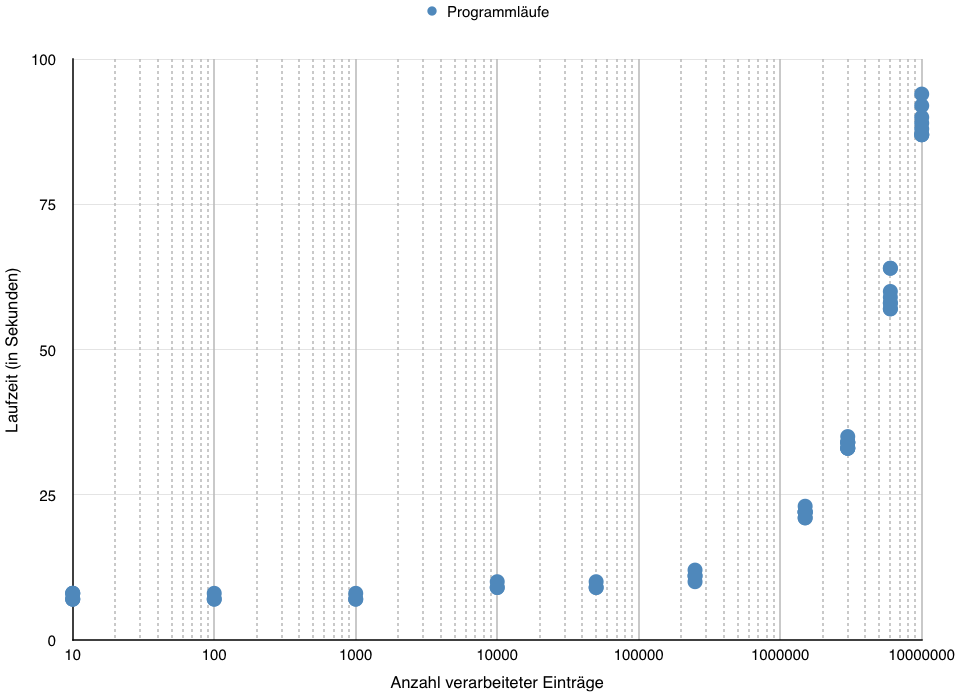
\includegraphics[width=1\textwidth]{ErgebnisAnwendungstest.png}
	\caption{Streudiagram der Laufzeiten}
	\label{fig:Streudiagram}
\end{figure}

\begin{table}
	\centering
	\begin{tabular}{| r | l | r | r |}
		\hline
		\rowcolor[HTML]{3531FF} 
		\multicolumn{1}{|l|}{\cellcolor[HTML]{4F88BB}{\color[HTML]{FFFFFF} {\bf \#}}} & \multicolumn{1}{l|}{\cellcolor[HTML]{4F88BB}{\color[HTML]{FFFFFF} {\bf Anzahl Einträge}}} & \multicolumn{1}{l|}{\cellcolor[HTML]{4F88BB}{\color[HTML]{FFFFFF} {\bf Dateigröße}}} & \multicolumn{1}{l|}{\cellcolor[HTML]{4F88BB}{\color[HTML]{FFFFFF} {\bf Laufzeit}}} \\ \hline
		1 & $10$ & 1,6 \ac{KB} & 7,4 \\  \hline
		2 & $100$ & 17,0 \ac{KB} & 7,1 \\ \hline
		3 & $1000$ & 157,0 \ac{KB} & 7,3 \\  \hline \hline
		4 & $10^4$ & 1,6 \ac{MB} & 9,1 \\  \hline
		5 & $5\times10^4$ & 7,7 \ac{MB} & 9,1 \\  \hline
		6 & $2,5\times10^5$ & 39,0 \ac{MB} & 11,0 \\  \hline
		7 & $1,5\times10^6$ & 231,0 \ac{MB} & 21,7 \\  \hline
		8 & $3\times10^6$ & 461,0 \ac{MB} & 33,7 \\  \hline
		9 & $6\times10^6$ & 921,0 \ac{MB} & 59,5 \\  \hline \hline
		10 & $10^7$ & 1,5 \ac{GB} & 88,9 \\  \hline
	\end{tabular}
	\caption{Durchschnittliche Laufzeiten (in Sekunden) für gegebene Datenmenge}
	\label{tbl:DurchschnittlicheLaufzeiten}
\end{table}

Die visuelle Darstellung lässt einen stärkeren Zusammenhang zwischen den beiden Größen $x$ und $y$ vermuten. Aus diesem Grund werden, die durch den Anwendungstest erhobenen Daten, genauer betrachtet.

Da die Tests auf der in \autoref{sec:InstallationHadoop} erwähnten \ac{VM} durchgeführt wurden, können die im folgenden getroffenen Aussagen vom späteren produktiven Betrieb abweichen. Aus diesem Grund sollten vor Inbetriebnahme der Anwendung weitere Tests auf einem System ähnlich dem Produktivsystem durchgeführt werden, um aussagekräftigere Daten zu erhalten.

\subsection{Analyse der Laufzeiten}\label{subsec:Laufzeitanalyse}
Die im Anwendungstest erhobenen Laufzeiten sollen nun weiter analysiert werden. Hierfür soll zunächst das Ausmaß des \textit{linearen} Zusammenhangs zwischen der Anzahl der verarbeiteten Einträge und der Laufzeit ermittelt werden. Gerald und Susanne Teschl definieren die, nach dem englischen Mathematiker Karl Pearson (1857 - 1936) benannte, Kennzahl wie folgt:

\flqq Gegeben seien die Wertepaare $(x_1,y_1), \dots,(x_n,y_n)$, wobei nicht alle $x_i$ gleich sind bzw. nicht alle $y_i$ gleich sind. Die Zahl
\begin{equation*}
r_{xy} = \frac{s_{xy}}{s_x \cdot s_y}
\end{equation*} 
heißt \textbf{(empirischer) Korrelationskoeffizient} oder \textbf{Pearson'scher Korrelationskoeffizient}. Dabei ist
\begin{equation*}
s_{xy} = \frac{1}{n-1} \displaystyle\sum_{i=1}^{n} (x_i - \bar{x})(y_i - \bar{y})
\end{equation*}
die \textbf{(empirische) Kovarianz}, $\bar{x}$, $\bar{y}$ sind die arithmetischen Mittelwerte und
\begin{equation*}
s_x = \sqrt{\frac{1}{n-1} \displaystyle\sum_{i=1}^{n} (x_i - \bar{x})^2}, \quad s_y = \sqrt{\frac{1}{n-1} \displaystyle\sum_{i=1}^{n} (y_i - \bar{y})^2}
\end{equation*}
sind die (empirischen) Standardabweichungen der $x_i$ bzw. der $y_i$-Werte.\frqq\footcite[S. 213]{Teschl.2014}

Der Pearson'sche Korrelationskoeffizient liegt immer zwischen $-1$ und $+1$. Je näher $r_{xy}$ an $-1$ oder $1$ liegt, desto genauer konzentrieren sich die Datenpunkte auf einer Geraden. Zudem spricht man bei einem Korrelationskoeffizienten $r_{xy}>0$ von einer \textbf{positiven (linearen) Korrelation}.\footcite[Vgl.][S. 214]{Teschl.2014}

Nach Anwendung der eben definierten Gleichungen auf die, durch den Anwendungstest, ermittelten Werte, ergibt sich ein Wert von $r_{xy} \approx 0,9982$. Daraus folgt eine starke, lineare Korrelation zwischen der Laufzeit und der Anzahl der verarbeiteten Einträge.

Basierend auf dieser Abhängigkeit lässt sich, durch die sog. \textbf{Regressionsanalyse}, eine Funktion bestimmen, mit welcher, die zu erwartende Laufzeit der Anwendung, in Abhängigkeit zur Menge der zu verarbeitenden Daten, approximiert werden kann.

Bei der \textbf{linearen Regression} wird eine Funktion der Form $y = f(x) = kx + d$ gesucht (der sog. \textbf{Regressionsgeraden}), welche der folgenden Definition gerecht wird:

\flqq Die Gerade $f(x) = kx + d$, für die
\begin{equation*}
\displaystyle\sum_{i=1}^{n} (y_i - f(x_i))^2
\end{equation*}
minimal wird, ist gegeben durch
\begin{equation*}
k = r_{xy} \frac{s_y}{s_x}, \quad \quad d = \bar{y} - k\bar{x}.
\end{equation*}
Hier ist $r_{xy}$ der empirische Korrelationskoeffizient, $\bar{x}$, $\bar{y}$ sind die arithmetischen Mittelwerte und $s_x$, $s_y$ die Standardabweichungen der Stichprobenwerte $x_i$ bzw. $y_i$.\frqq\footcite[216]{Teschl.2014}

Daraus ergeben sich, basierend auf den ermittelten Testdaten, die Werte $k \approx 8,199 \times 10^{-6}$, $d \approx 8,418$, und die \autoref{equ:Laufzeit}, für die Berechnung der Laufzeit.

\begin{flalign}
&&  && t_e = f(x) = 8,199 \times 10^{-6}x + 8,418 && \{x \in \mathbb{N}\} \label{equ:Laufzeit}
\end{flalign}

\newpage
\autoref{fig:VerlaufRegressionsgerade} zeigt den Verlauf der Regressionsgeraden durch die Testdaten.

\begin{figure}[h]
	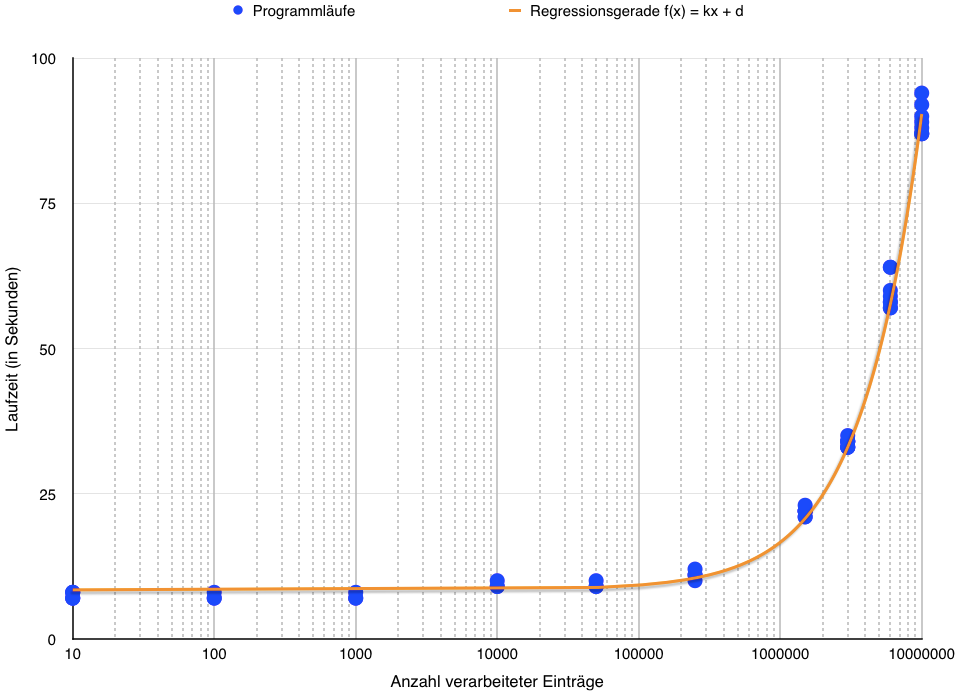
\includegraphics[width=1\textwidth]{Laufzeitanalyse.png}
	\caption{Verlauf der Regressionsgeraden}
	\label{fig:VerlaufRegressionsgerade}
\end{figure}

Um die ermittelte Funktion zu testen, wird nun zunächst die Laufzeit für die Verarbeitung von $2 \times 10^7$ Einträgen mit \autoref{equ:Laufzeit} berechnet. Anschließend wird die Anwendung mit der entsprechenden Anzahl von Einträgen zehn mal ausgeführt (siehe \autoref{lis:Laufzeit20Mio}), und die durchschnittliche Laufzeit mit der Berechnung verglichen. Die Dateigröße, bei $2 \times 10^7$ Einträgen, beträgt 3 \ac{GB}. \\

\begin{lstlisting}[language=Bash,caption=Laufzeiten mit $2 \times 10^7$ Einträgen,label=lis:Laufzeit20Mio]
Runtime: 185
Runtime: 171
Runtime: 166
Runtime: 174
Runtime: 166
Runtime: 172
Runtime: 170
Runtime: 170
Runtime: 171
Runtime: 171
\end{lstlisting}

Die berechnete Laufzeit beträgt $t_e = 172,398$. Die durchschnittliche Laufzeit, bei 20 Mio. Einträgen, beträgt $171,6$. Die berechnete Laufzeit weicht lediglich $\approx 0,46\%$ vom Durchschnitt ab, was die Richtigkeit der Funktion hinreichend bestätigt.

\subsubsection{Randbemerkung zur Berechnung der Laufzeit}
Bei Tests mit weiteren Logfiles, welche eine abweichende Formatierung hatten, konnte festgestellt werden, dass die berechnete Laufzeit nur dann zutreffend ist, wenn sowohl Mapper als auch Reducer die gleiche Anzahl an Datensätzen verarbeiten muss.

Angenommen die Logeinträge einer Datei erstrecken sich über mehr als eine Zeile. Um unnötige Informationen direkt zu filtern, wird die \textit{SKIP} Anweisung für den \textit{PatternMapper} aktiviert. Dies hat zur Folge, dass nur die Zeilen verarbeitet werden, welche das gesucht Muster enthalten. Wird nun ein Logfile mit $7 \times 10^6$ Zeilen verarbeitet, wo nur $3 \times 10^5$ Zeilen den regulären Ausdruck erfüllen können, hat dies zur Folge, dass der Reducer wesentlich weniger Datensätze zu verarbeiten hat. Die Laufzeit ist entsprechend geringer.

Da es, ohne eine bereits durchgeführte Analyse, nicht möglich ist zu wissen, wie viele Zeilen dem Muster gerecht werden können, handelt es sich bei der Berechneten Laufzeit um die maximale, durchschnittliche Laufzeit.

\subsection{Berechnung der maximalen Datenmenge}
Die Logfiles, der in \autoref{subsec:Infrastruktur} beschriebenen Infrastruktur, befinden sich in einer stündlichen Rotation, d.h., dass jede Stunde die aktuellen Logfiles verschoben und neue angelegt werden. Für alle verschobenen Logfiles ist zusätzlich die Durchführung einer Analyse notwendig.

Basierend auf der in \autoref{subsubsec:PL001} formulierten Produktleistung \textbf{PL001}, darf die Laufzeit der Analyse lediglich ein Fünftel des Intervalls betragen. Aus dieser Definition ergibt sich, für die Analyse der stündlich rotierenden Logfiles, eine Laufzeit von $t_e \leq 720$.

Durch die Anwendung von \autoref{equ:Laufzeit} lässt sich, durch eine Umformung nach $x$, die maximale Datenmenge, für die zu analysierenden Logfiles errechnen.

\begin{flalign*}
&& 720 &= 8,199 \times 10^{-6} x + 8,418 &&| - 8,418 \\
&& 720 - 8,418 &= 8,199 \times 10^{-6} x &&| \div 8,199 \times 10^{-6} \\
&& \frac{720 - 8,418}{8,199 \times 10^{-6}} &= x \\
&& 86.788.877 &\approx x
\end{flalign*}

Die Produktleistung lässt sich somit erfüllen, solange die stündliche generierte Datenmenge $x \leq 86.788.877$ beträgt.

Ein Weg diesen Schwellenwert zu umgehen bietet die Möglichkeit Daten zu Streamen. Dabei können Dateien entweder nach HDFS oder direkt als Eingabe übertragen werden. Der Verarbeitungsprozess verändert sich jedoch sehr stark im vergleich zur normalen Datenverarbeitung. Die Laufzeit wird durch den Veränderten Prozess ebenfalls beeinflusst.

Aufgrund dieser Komplexität und der Tatsache, dass Streaming kein teil der definierten Anforderungen ist, wir dieser Punkt nicht weiter verfolgt.

%<IDEE: Es wurde eine formel angegeben, welche aussage über die maximale ausführungsdauer gibt...eventuell lassen sich diese beiden formeln verbinden (also eine Formel die aussage gibt über den maximal möglichen intervall für eine bestimmte datenmenge \autoref{equ:MinInterval})>

%\begin{figure}
%	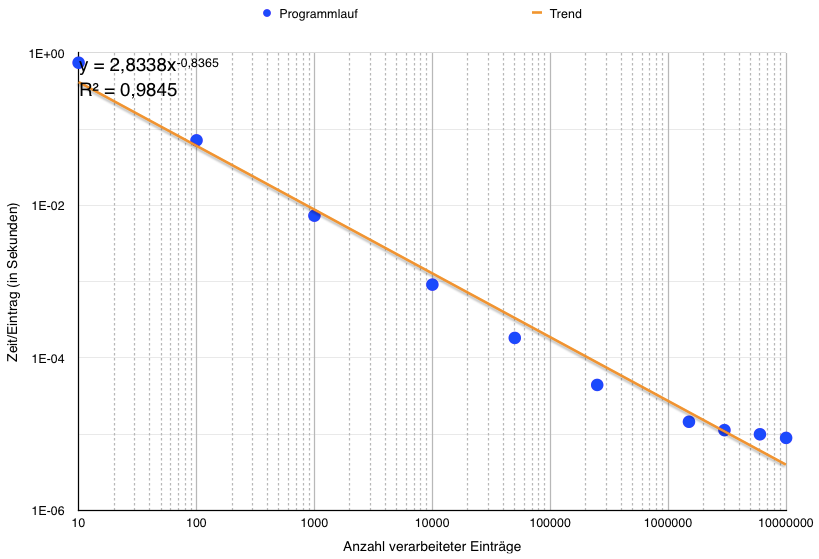
\includegraphics[width=1\textwidth]{Zeit_Pro_Eintrag.png}
%	\caption{Verarbeitungszeit pro Eintrag}
%	\label{fig:VerarbeitungszeitProEintrag}
%\end{figure}

%<Dokumentation der Tests mit unterschiedlich großen Datenmengen (10 Logeinträge bis 10.000.000 Einträge). Grafische Darstellung der Laufzeiten. Jede Stufe min. 10 mal ausführen und Ausführungszeit Nottieren/Dokumentieren. In Kapitel 6 Erkenntnisse aus den Tests aufarbeiten>